%% \documentclass[unicode, 11pt]{beamer}
%% \usepackage{luatexja}
%% \usepackage[ipaex]{luatexja-preset}

%%%%%%%%%% for uplatex users %%%%%%%
\documentclass[aspectratio=169,
  14pt,xcolor=dvipsnames,table,professional font,dvipdfmx]{beamer}
%\usepackage[uplatex,deluxe]{otf}
\usepackage{bxdpx-beamer}
\usepackage{pxjahyper}
\usepackage{minijs}
\usepackage{pgf}
\usepackage{booktabs}
\usepackage{listings}
\usepackage{listinglangd}
\usepackage{color}
\usepackage{comment}
%\usepackage{dejavu}
\definecolor{mygreen}{rgb}{0,0.6,0}
\definecolor{mygray}{rgb}{0.5,0.5,0.5}
\definecolor{mymauve}{rgb}{0.58,0,0.82}

\usepackage{etoolbox}
\usepackage{xcolor}
\usepackage{listings}

\newtoggle{InString}{}% Keep track of if we are within a string
\togglefalse{InString}% Assume not initally in string

\newcommand*{\ColorIfNotInString}[1]{\iftoggle{InString}{#1}{\color{mygreen}#1}}%
\newcommand*{\ProcessQuote}[1]{#1\iftoggle{InString}{\global\togglefalse{InString}}{\global\toggletrue{InString}}}%
\lstset{literate=%
    {"}{{{\ProcessQuote{"}}}}1% Disable coloring within double quotes
    {'}{{{\ProcessQuote{'}}}}1% Disable coloring within single quote
    {0}{{{\ColorIfNotInString{0}}}}1
    {1}{{{\ColorIfNotInString{1}}}}1
    {2}{{{\ColorIfNotInString{2}}}}1
    {3}{{{\ColorIfNotInString{3}}}}1
    {4}{{{\ColorIfNotInString{4}}}}1
    {5}{{{\ColorIfNotInString{5}}}}1
    {6}{{{\ColorIfNotInString{6}}}}1
    {7}{{{\ColorIfNotInString{7}}}}1
    {8}{{{\ColorIfNotInString{8}}}}1
    {9}{{{\ColorIfNotInString{9}}}}1
}

\lstset{ %
  frame=single,
  backgroundcolor={\color{black}}, %\pgfsetfillopacity{0.85}},
  %xleftmargin=.05\textwidth, %xrightmargin=.1\textwidth,
  %backgroundcolor=\color{white},   % choose the background color; you must add \usepackage{color} or \usepackage{xcolor}; should come as last argument
  %basicstyle=\tiny\ttfamily,                % the size of the fonts that are used for the code
  basicstyle=\footnotesize\ttfamily,
  breakatwhitespace=false,         % sets if automatic breaks should only happen at whitespace
  breaklines=true,                 % sets automatic line breaking
  captionpos=b,                    % sets the caption-position to bottom
  commentstyle=\color{OwlGreen},    % comment style
  deletekeywords={...},            % if you want to delete keywords from the given language
  escapeinside={\%*}{*)},          % if you want to add LaTeX within your code
  extendedchars=true,              % lets you use non-ASCII characters; for 8-bits encodings only, does not work with UTF-8
  % frame=single,	              % adds a frame around the code
  keepspaces=true,                 % keeps spaces in text, useful for keeping indentation of code (possibly needs columns=flexible)
  keywordstyle=\color{OwlRed},       % keyword style
  language={D},                 % the language of the code
  %morekeywords={*,...},            % if you want to add more keywords to the set
  numbers=left,                    % where to put the line-numbers; possible values are (none, left, right)
  numbersep=5pt,                   % how far the line-numbers are from the code
  numberstyle=\tiny\color{mygray}, % the style that is used for the line-numbers
  rulecolor=\color{mygray},         % if not set, the frame-color may be changed on line-breaks within not-black text (e.g. comments (green here))
  showspaces=false,                % show spaces everywhere adding particular underscores; it overrides 'showstringspaces'
  showstringspaces=false,          % underline spaces within strings only
  showtabs=false,                  % show tabs within strings adding particular underscores
  stepnumber=1,                    % the step between two line-numbers. If it's 1, each line will be numbered
  stringstyle=\color{mymauve},     % string literal style
  tabsize=2,	                     % sets default tabsize to 2 spaces
  title=\lstname                   % show the filename of files included with \lstinputlisting; also try caption instead of title
}



\AtBeginSection[]{
    \begin{frame}
        \tableofcontents[currentsection]
    \end{frame}
}

%\renewcommand{\kanjifamilydefault}{\gtdefault}% 既定をゴシック体に
\usepackage{default}

%\usepackage{biblatex}

\usepackage[style=authoryear]{biblatex}
\renewcommand*{\nameyeardelim}{\addcomma\addspace}
%\bibliographystyle{IEEEbib}
\bibliography{refs}


%\usetheme{metropolis}           % Use metropolis theme
\usepackage{theme}

%\usecolortheme{dove}
% \usecolortheme{orchid}
% \usepackage{transparent}
% \usepackage{tikz}
\usecolortheme{owl}

%% NOTE: colors http://www2.informatik.uni-freiburg.de/~frank/latex-kurs/latex-kurs-3/farben/Extra-Farben.pdf
%% \setbeamertemplate{frametitle}{\vspace{0.5em}\color{black}\insertframetitle}
%% \setbeamercolor*{normal text}{fg=black,bg=white}
%% \setbeamercolor*{alerted text}{fg=Plum}
%% \setbeamercolor*{example text}{fg=MidnightBlue} % VioletRed}
%% \setbeamercolor*{structure}{fg=black}
%% %% setting for blocks without box
%% %\setbeamercolor*{block title}{parent=structure}
%% \setbeamerfont{block title}{size={}}


%\usetheme{Madrid}
\title{grain}
\subtitle{D Language for Deep Learning}
\date{4. Oct. 2018}
\author{Shigeki Karita}
\institute{ML Meetup KANSAI \#3 LT}
\begin{document}

% タイトル用の背景
\setbeamercolor{bgcolor}{fg=white,bg=black}
%% \setbeamercolor{normal text}{fg=white,bg=black!90}
%% \setbeamertemplate{frametitle}{\vspace{0.5em}\color{white}\insertframetitle}
%% \setbeamercolor{normal text}{fg=white,bg=black!90}
%% \setbeamercolor{alerted text}{fg=Plum}
%%
\setbeamercolor{example text}{fg=Cerulean} % VioletRed}
%% \setbeamercolor{structure}{fg=white}
%% \setbeamercolor{framesubtitle}{fg=white}
%% \setbeamercolor{block title}{parent=structure,bg=black!60}
%% \setbeamercolor{block body}{fg=black,bg=black!10}
%% \setbeamercolor{block title alerted}{parent=alerted text,bg=black!15}
%%
\setbeamercolor{block title example}{parent=example text,fg=Cerulean} %,bg=black!15}

%% \setbeamercolor{item projected}{use=item,fg=black,bg=item.fg!35}

%% \setbeamercolor*{palette primary}{use=structure,fg=structure.fg}
%% \setbeamercolor*{palette secondary}{use=structure,fg=structure.fg!95!black}
%% \setbeamercolor*{palette tertiary}{use=structure,fg=structure.fg!90!black}
%% \setbeamercolor*{palette quaternary}{use=structure,fg=structure.fg!95!black,bg=black!80}


%% setting for blocks without box
%\setbeamercolor*{block title}{parent=structure}
%\setbeamerfont{block title}{size={}}


\usebackgroundtemplate{%
  \begin{beamercolorbox}[wd=1.1\paperwidth,ht=\paperheight]{bgcolor}
  \begin{picture}(400,400)(-30, -30)
    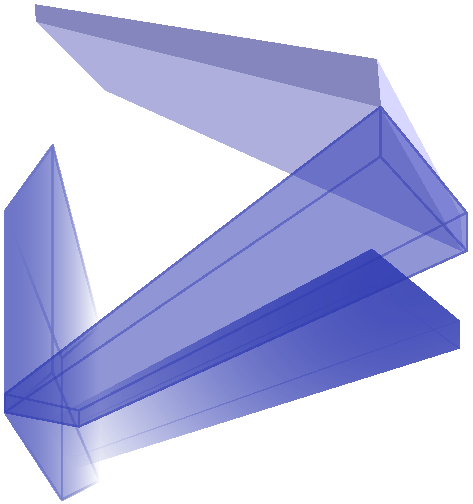
\includegraphics[height=1.1\paperheight]{fig/grain2.pdf}
  \end{picture}
  \end{beamercolorbox}
}


\maketitle

\usebackgroundtemplate{%
  \begin{beamercolorbox}[wd=1.1\paperwidth,ht=\paperheight]{bgcolor}
    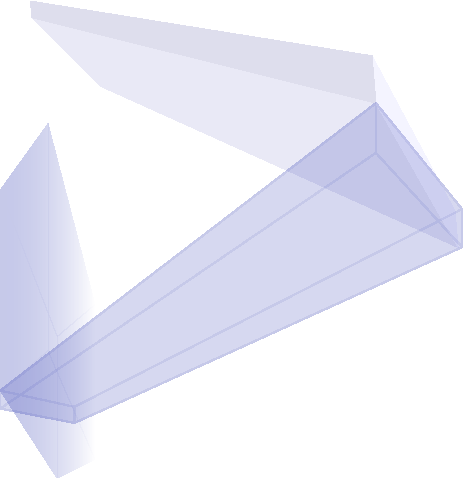
\includegraphics[height=\paperheight]{fig/grain_opac.pdf}
  \end{beamercolorbox}
}


%% \begin{frame}{Table of contents}
%%   \tableofcontents
%% \end{frame}

%\section{Why D}
\begin{frame}{\alert{D L}anguage for \alert{D}eep \alert{L}earning}
  \begin{alertblock}{language}
    \begin{itemize}
    \item \textbf{like C++}: fast, strongly typed, LLVM/GCC backend
    \item \textbf{like Python}: simple, lightweight, jupyter support
    \end{itemize}
  \end{alertblock}
  %\pause
  \begin{exampleblock}{libraries\footnote{\url{https://github.com/libmir}}}
    \begin{itemize}
    \item \textbf{mir}: N-dim fast algorithm, numpy-like APIs
    \item \textbf{dcompute}: CUDA kernel DSL
    \end{itemize}
  \end{exampleblock}
\end{frame}

\begin{frame}{grain}
  \begin{alertblock}{deep learning framework for D}
    \begin{itemize}
    \item \alert{\url{https://github.com/ShigekiKarita/grain}}
    \item boost software license 1.0
    \end{itemize}
  \end{alertblock}
  \begin{exampleblock}{philosophy}
    \begin{itemize}
    \item \textbf{DYNAMIC}: like chainer and pytorch
    \item \textbf{SAFE}: statically typed variable and function
    \item \textbf{LIGHT}: simple like Python, small like C++
    \item \textbf{FAST}: mir and CUDA backend
    \end{itemize}
  \end{exampleblock}
\end{frame}

\begin{frame}[fragile]{grain is \alert{dynamic}}
like chainer ...
  \begin{lstlisting}[language=D]
foreach (epoch; 0 .. 10) {
  foreach (i; niter.permutation) {
    auto xs = inputs[i].variable;
    auto ts = targets[i].variable;
    auto ys = model(xs);
    auto loss = crossEntropy(ys, ts);
    auto acc = accuracy(ys, ts);
    model.zeroGrad();
    loss.backward();
    optimizer.update();
  }
}\end{lstlisting}
\end{frame}

\begin{frame}[fragile]{grain is \alert{safe}}
but statically typed and optimized.
  \begin{lstlisting}[language=D,basicstyle=\footnotesize\ttfamily]
foreach (epoch; 0 .. 10) {
  foreach (i; niter.permutation) {
    Variable!(float, 3, HostStorage) xs = inputs[i].variable;
    Variable!(int, 1, HostStorage) ts = targets[i].variable;
    Variable!(float, 2, HostStorage) ys = model(xs);
    Variable!(float, 0, HostStorage)loss =crossEntropy(ys, ts);
    float acc = accuracy(ys, ts);
    model.zeroGrad();
    loss.backward();
    optimizer.update();
  }
}\end{lstlisting}
\end{frame}

\begin{frame}[fragile]{grain is \alert{safe}}
  every function is statically typed and optimized.
  \begin{lstlisting}[language=D,basicstyle=\footnotesize\ttfamily]
struct Sigmoid(T, size_t dim) {
  Variable!(T, dim, HostStorage) y;

  nothrow forward(Variable!(T, dim, HostStorage) x) {
    auto y = x.sliced.map!(a => tanh(a * 0.5) * 0.5 + 0.5)
              .slice.variable(x.requiresGrad);
    if (x.requiresGrad) this.y = y;
    return y;
  }
  nothrow backward(Variable!(T, dim, HostStorage) gy) {
    auto ys = this.y.sliced;
    return slice((1.0 - ys) * ys * gy.sliced).variable;
  }
  mixin FunctionCommon; // inject type checking
}\end{lstlisting}
\end{frame}

\begin{frame}{grain is \alert{safe}}
  \begin{alertblock}{Chainer/PyTorch issue}
  \begin{itemize}
  \item runtime overhead
    \begin{itemize}
    \item for-loop, dynamic dispatch, func call
    \end{itemize}
  \item runtime error:
    \begin{itemize}
    \item type error, exception safety, memory leak
    \end{itemize}
  \end{itemize}
  \end{alertblock}
  \begin{exampleblock}{D solution}
    \begin{itemize}
    \item template based code generation
    \item compile-time type/error checking
    \end{itemize}
  \end{exampleblock}
\end{frame}

\begin{frame}[fragile]{grain is \alert{a lightweight framework}}
  Jupyter notebook support
  \footnote{\alert{\url{https://github.com/ShigekiKarita/grain/blob/master/tutorial.ipynb}}}
  \begin{figure}[b]
	\centering
	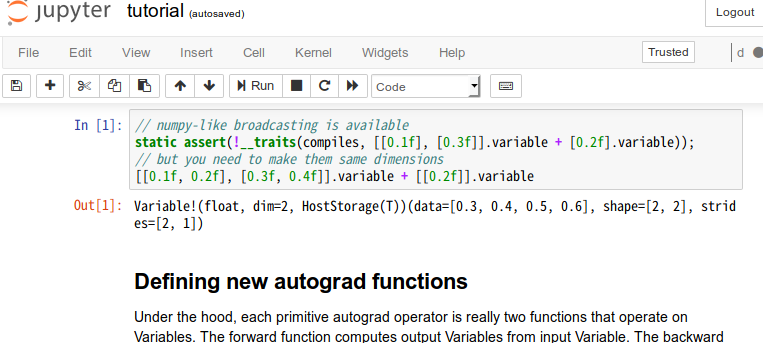
\includegraphics[height=0.6\textheight]{./fig/jupyterd.png}
  \end{figure}
  \scriptsize
\end{frame}

\begin{frame}[fragile]{grain is \alert{a lightweight framework}}
  smaller code and footprint
  \begin{table}
	\begin{tabular}{lrrr}
      \toprule
      framework   & code lines & lib size [mb] & lib type  \\
      \midrule
      \textbf{grain} &  \textbf{12,431} & \textbf{0.6}  & \textbf{static} \\
      chainer    & 162,106 & 6 & python code \\
      pytorch    & 193,754 & 911 &dynamic \\
      tensorflow & 130,475 & 285 & dynamic  \\
      \bottomrule
	\end{tabular}
  \end{table}
  smaller exe file (MNIST : 1.8MB, CIFAR: 2.3MB)
\end{frame}

\begin{frame}{grain is as \alert{fast} as other frameworks}
    \begin{table}
	\begin{tabular}{lllrr}
      \toprule
      task & backend  & framework & train iter/sec \\
      \midrule
      mnist & CUDA & grain      & 270 \\
            &      & chainer    & 340 \\
            &      & pytorch    & 200 \\
      \midrule
            & CPU  & grain      & 160 \\
            &      & chainer    &  95 \\
            &      & pytorch    & 110 \\
      \bottomrule
	\end{tabular}
    \end{table}
    \begin{itemize}
      \item chainer 4.5.0, pytorch 0.4.1, MKL2018, CUDA9, CUDNN7
      \item pytorch is built from source. modified official scripts to be fair.
    \end{itemize}
\end{frame}

\begin{frame}{grain is as \alert{fast} as other frameworks}
    \begin{table}
	\begin{tabular}{lllrr}
      \toprule
      task & backend  & framework & train iter/sec \\
      \midrule
      ptb   & CUDA & grain      & 3.1  \\
            &      & chainer    & 3.4 \\
            &      & pytorch    & 12 \\
      \midrule
            & CPU  & grain      & 1.2 \\
            &      & chainer    & 2.1 \\
            &      & pytorch    & 2.4 \\
      \bottomrule
	\end{tabular}
    \end{table}
    \begin{itemize}
      \item chainer 4.5.0, pytorch 0.4.1, MKL2018, CUDA9, CUDNN7
      \item pytorch is built from source. modified official scripts to be fair.
    \end{itemize}
\end{frame}


\begin{frame}{grain: summary} % Thank you for your attention}
  \large
  \textbf{deep learning framework for \alert{D language}}
  \vspace{1em}
  \begin{itemize}
    \large
  \item \textbf{DYNAMIC}: like chainer and pytorch
  \item \textbf{SAFE}: statically typed variable and function
  \item \textbf{LIGHT}: simple like Python, small like C++
  \item \textbf{FAST}: mir and CUDA backend
  \end{itemize}
\end{frame}

{
  \usebackgroundtemplate{%
    \begin{beamercolorbox}[wd=1.1\paperwidth,ht=\paperheight]{bgcolor}
      \begin{picture}(300,300)(-200, -100)
        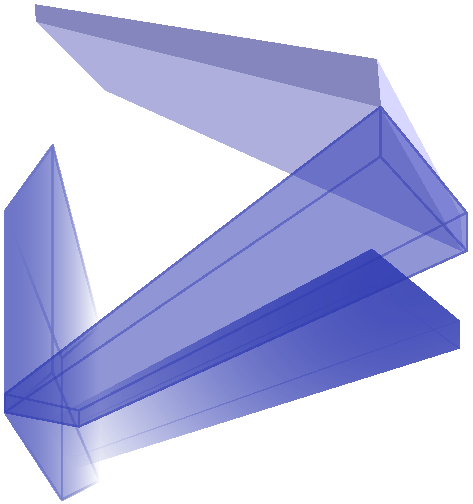
\includegraphics[height=0.5\paperheight]{fig/grain2.pdf}
      \end{picture}
    \end{beamercolorbox}
}
\begin{frame}{} % Thank you for your attention}
    %% \begin{alertblock}{grain: deep learning framework for D language}
    %% \begin{itemize}
    %% \item \textbf{DYNAMIC}: like chainer and pytorch
    %% \item \textbf{SAFE}: statically typed variable and function
    %% \item \textbf{LIGHT}: simple as Python, small as C++
    %% \item \textbf{FAST}: mir and CUDA backend
    %% \end{itemize}
  %% \end{alertblock}
  \vspace*{10em}
    \begin{center}
      \large
      Thanks for your attention
      \\
      \alert{\url{https://github.com/ShigekiKarita/grain}}
    \end{center}
\end{frame}
}

\begin{frame}{examples}
  \begin{itemize}
  \item Image recognition (mnist, cifar)
  \item Language modeling (shakespere, ptb)
  \item WIP
  \begin{itemize}
  \item Reinforcement learning (cartpole)
  \item Speech recognition (librispeech)
  \item Machine translation (anki)
  \end{itemize}
  \end{itemize}
\end{frame}

\begin{frame}{future work}
  \begin{itemize}
  \item probabilistic programming
  \item lazy evaluation mode
  \item low resource environment (RasberryPi)
  \end{itemize}
\end{frame}

%% %%%%%%%%%%%%%%%%%%%%%%%%%%%%%%%%%%%%%%%%%%%%%%%%%%%%%
%% \begin{frame}
%% %\frametitle{References}
%% % This prints the bibliography on the slide
	
%% \begin{small}
%% \printbibliography
%% \end{small}
%% \end{frame}

\end{document}

